\chapter{Introduction to Model-Based Systems Engineering}

\begin{lernziele}
After this chapter, you will understand the difference between document-centric development and model-based development. You will be able to explain what \gls{mbse} means, which information a system model holds, and why a central model is useful for complex projects. You will be able to describe the benefit of MBSE using the autonomous indoor robot as an example, recognize common misunderstandings, and structure first model content for your own robot project.
\end{lernziele}

\section{Introduction}
The previous chapter looked at systems engineering as a way of thinking: a technical system is not just a collection of parts, but an interplay of requirements, functions, components, interfaces, behavior, tests, and operating environment. This way of thinking already helps, even if you only work with text, tables, and sketches.

In real projects, though, a practical problem soon appears. Information lives in many places. Requirements sit in a Word document or a spreadsheet. Architecture decisions get drawn in PowerPoint. Interfaces get discussed in emails. Test cases sit in a test management tool. Software gets developed in Git. Tasks sit in Jira or a similar tool. Meeting notes end up somewhere in the project folder.

As long as the project stays small, this can work. Once several people get involved and requirements start changing, it gets hard. Which version is current? Which component satisfies which requirement? Which tests check obstacle detection? Which ROS2 node uses which sensor data? (A node is a software module; a topic is a communication channel between nodes -- more on this later in this chapter.) Which documents need updating when the robot gets a new camera?

This is exactly where \gls{mbse} starts. Model-Based Systems Engineering means that a model becomes the central carrier of the system's key information. The model does not replace everything. It does not replace the code, every calculation, or every conversation. But it connects the decisive pieces of information so that relationships stay traceable.

\begin{praxisbox}
For the indoor robot, one requirement could be: \enquote{The robot must detect obstacles in time and stop safely.} In the MBSE model, this requirement can be linked to a function \enquote{detect obstacle}, to a lidar sensor, to safety logic, to a ROS2 node, and to a test case. This lets the team see later which parts are affected when the requirement changes.
\end{praxisbox}

\section{Document-Centric Development}
Document-centric development means that project information lives mainly in separate documents. These can be text files, spreadsheets, presentations, diagram images, emails, or tickets. This way of working is common because it is easy to start. Almost anyone can write a document, fill in a table, or draw a diagram.

The start is comfortable. A team builds a requirements list in Excel. The architecture gets sketched in PowerPoint. A developer describes an interface in a Markdown document. A tester sets up test cases in a table. For a very small project, this is often enough.

As complexity grows, though, typical problems appear:

\begin{itemize}
    \item Information gets stored more than once.
    \item Different documents contradict each other.
    \item Changes do not propagate everywhere.
    \item Diagrams look current but hold outdated content.
    \item Relationships between requirements, architecture, and tests are hard to see.
    \item New team members need a long time to understand the project's current state.
    \item Decisions become almost impossible to trace later.
\end{itemize}

\subsection{Example: A Changed Camera}
Suppose the indoor robot gets a depth camera instead of a simple camera. In a document-centric setting, this change can touch many documents:

\begin{itemize}
    \item the bill of materials
    \item the architecture diagram
    \item the description of the sensors
    \item the interface specification
    \item the power consumption estimate
    \item the software description of image processing
    \item the data protection assessment
    \item the test cases for people detection
\end{itemize}

If even one of these documents gets forgotten, a contradiction appears. Maybe the architecture still shows the old camera while the interface specification already describes the new one. Maybe the test team still tests with old image formats. Maybe no one notices that the new camera draws more power and shortens battery life.

\subsection{The Silent Cost of Synchronization}
In document-centric projects, a large share of the work is synchronization. People must compare documents, pass on changes, update tables, and ask which information is current. This effort is often invisible, but it costs time and creates errors.

A typical sentence in such projects is: \enquote{Where is the current version?} Another is: \enquote{Didn't we already change that?} Both are warning signs. They show that project knowledge is not organized reliably.

\section{What Does Model-Based Development Mean?}
Model-based development means that key information about the system lives in a model. A model is more than a drawing. It consists of model elements and the relationships between them.

A model element can be, for example:

\begin{itemize}
    \item a requirement
    \item a stakeholder
    \item a function
    \item a system element (\texttt{part def}) or subsystem
    \item an interface
    \item a data flow
    \item a state
    \item a test case
    \item a ROS2 node as a later implementation unit
\end{itemize}

The relationships matter at least as much as the elements themselves. A requirement can be satisfied by a function. A function can be realized by a component. A component can have an interface. A test case can verify a requirement. A ROS2 node can be part of a software architecture and exchange data over a topic.

\subsection{Model Instead of Picture}
This point matters especially for beginners: a diagram is not automatically a model. A diagram can just be a picture. Drawing boxes and arrows in PowerPoint may look like an architecture model. But the boxes know nothing about each other. If the same block appears in three diagrams, in PowerPoint these are three separate graphical objects.

In a real modeling tool, by contrast, a diagram is a view onto model elements. The system element \texttt{NavigationSystem} exists in the model. It can appear in several diagrams. If its name changes, the change should become visible everywhere. If a requirement is linked to this block, the tool can show that relationship.

\begin{hinweisbox}
An MBSE model is not good because it contains pretty diagrams. It is good when it answers important questions: What must the system do? Which parts satisfy which requirements? What interfaces exist? What happens on a change? How is fulfilment demonstrated?
\end{hinweisbox}

\subsection{The Model as a Shared Information Base}
The goal of an MBSE model is a shared information base. Everyone involved should not work in separate document worlds; instead, they should be able to access one consistent system description. This does not mean that everyone must see every detail. A project manager may care about requirements, risks, and milestones. A software developer may care about interfaces, data flows, and ROS2 nodes. A tester may care about requirements and test cases. The model can offer different views for different roles. Figure~\ref{fig:kap02-dokumentenzentriert-vs-modellbasiert} contrasts this difference between a loose document collection and a central model once more, in pictures.

\begin{figure}[H]
  \centering
  \adjustbox{max width=\linewidth,max totalheight=0.6\textheight}{% =====================================================================
% Figure: Document-centric vs. model-based
% Belongs with chapter 2, section "Document-Centric Development" /
% "What Does Model-Based Development Mean?"
%
% Used in the book, e.g. in chapters_en/02_mbse.tex:
%
%   \begin{figure}[H]
%     \centering
%     % =====================================================================
% Figure: Document-centric vs. model-based
% Belongs with chapter 2, section "Document-Centric Development" /
% "What Does Model-Based Development Mean?"
%
% Used in the book, e.g. in chapters_en/02_mbse.tex:
%
%   \begin{figure}[H]
%     \centering
%     % =====================================================================
% Figure: Document-centric vs. model-based
% Belongs with chapter 2, section "Document-Centric Development" /
% "What Does Model-Based Development Mean?"
%
% Used in the book, e.g. in chapters_en/02_mbse.tex:
%
%   \begin{figure}[H]
%     \centering
%     \input{figures_en/fig_kap02_dokumentenzentriert_vs_modellbasiert}
%     \caption{Document-centric development with many loosely linked
%       documents, compared to a central, clearly linked system model.}
%     \label{fig:kap02-dokumentenzentriert-vs-modellbasiert}
%   \end{figure}
%
% Required packages (already loaded in main_en.tex): tikz
% Required TikZ libraries: positioning, arrows.meta, shadows, calc
% =====================================================================

\input{figures_en/fig_kap02_dokumentenzentriert_vs_modellbasiert.tikz}

%     \caption{Document-centric development with many loosely linked
%       documents, compared to a central, clearly linked system model.}
%     \label{fig:kap02-dokumentenzentriert-vs-modellbasiert}
%   \end{figure}
%
% Required packages (already loaded in main_en.tex): tikz
% Required TikZ libraries: positioning, arrows.meta, shadows, calc
% =====================================================================

\begin{tikzpicture}[
    every node/.style={font=\small},
    doc/.style={
        rectangle, rounded corners=1.5pt, draw=black!50, thick, dashed,
        minimum width=20mm, minimum height=8mm,
        align=center, fill=white, drop shadow, font=\tiny
    },
    modellbox/.style={
        rectangle, rounded corners=1.5pt, draw=green!40!black, thick,
        minimum width=26mm, minimum height=10mm,
        align=center, fill=green!15, drop shadow
    },
    req/.style={
        rectangle, rounded corners=1.5pt, draw=black!70, thick,
        minimum width=20mm, minimum height=8mm,
        align=center, fill=blue!12, drop shadow, font=\tiny
    },
    part/.style={
        rectangle, rounded corners=1.5pt, draw=green!40!black, thick,
        minimum width=20mm, minimum height=8mm,
        align=center, fill=green!15, drop shadow, font=\tiny
    },
    tool/.style={
        rectangle, rounded corners=1.5pt, draw=orange!60!black, thick,
        minimum width=20mm, minimum height=8mm,
        align=center, fill=orange!15, drop shadow, font=\tiny
    },
    test/.style={
        rectangle, rounded corners=1.5pt, draw=black!50, thick,
        minimum width=20mm, minimum height=8mm,
        align=center, fill=black!6, drop shadow, font=\tiny
    },
    stakeholder/.style={
        rectangle, rounded corners=1.5pt, draw=black!50, thick, dashed,
        minimum width=20mm, minimum height=8mm,
        align=center, fill=white, drop shadow, font=\tiny
    },
    chaos/.style={black!35, dashed, thin},
    clearlink/.style={-{Stealth[length=1.8mm]}, thick, black!55}
]

% --- Titles ---
\node[font=\bfseries\small] at (2.5,8.2) {Document-centric};
\node[font=\bfseries\small] at (11,8.2) {Model-based};

% --- Divider line ---
\draw[black!25, dashed] (6.55,-0.6) -- (6.55,8.0);

% --- Left side: loose documents, chaotically connected ---
\node[doc] (word) at (1,7)     {Word};
\node[doc] (excel) at (4,6.4)  {Excel};
\node[doc] (ppt)  at (1.8,5)   {PowerPoint};
\node[doc] (mail) at (4.3,3.8) {Email};
\node[doc] (tmt)  at (1.3,2.6) {Test Management\\Tool};
\node[doc] (git)  at (4,1.4)   {Git};
\node[doc] (jira) at (2,0.2)   {Jira};

\draw[chaos] (word) -- (excel);
\draw[chaos] (excel) -- (mail);
\draw[chaos] (mail) -- (git);
\draw[chaos] (git) -- (jira);
\draw[chaos] (jira) -- (tmt);
\draw[chaos] (tmt) -- (ppt);
\draw[chaos] (ppt) -- (word);
\draw[chaos] (word) -- (mail);
\draw[chaos] (excel) -- (tmt);
\draw[chaos] (git) -- (ppt);

% --- Right side: central model with clear relationships ---
\node[modellbox] (modell) at (11,4) {Model};

\node[stakeholder] (stake) at (11,6.4)    {Stakeholder};
\node[req]         (anf)   at (12.88,5.5) {Requirement};
\node[tool]        (code)  at (13.34,3.47){Code};
\node[test]        (test)  at (12.04,1.83){Test};
\node[part]        (schn)  at (9.96,1.83) {Interface};
\node[part]        (strukt)at (8.66,3.47) {Structure};
\node[part]        (funk)  at (9.12,5.5)  {Function};

\draw[clearlink] (modell) -- (stake);
\draw[clearlink] (modell) -- (anf);
\draw[clearlink] (modell) -- (code);
\draw[clearlink] (modell) -- (test);
\draw[clearlink] (modell) -- (schn);
\draw[clearlink] (modell) -- (strukt);
\draw[clearlink] (modell) -- (funk);

% --- Legend ---
% Boxes and labels are chained relative to the previous element (instead
% of fixed absolute offsets from leg1) so that labels of different
% lengths (e.g. "Structure/Function/Interface") do not overlap the next
% box.
\node[req, minimum width=6mm, minimum height=4mm, font=\tiny] (leg1) at (0.5,-2.2) {};
\node[right=1mm of leg1, font=\tiny, align=left] (lab1) {Requirement};
\node[part, minimum width=6mm, minimum height=4mm, font=\tiny, right=6mm of lab1] (leg2) {};
\node[right=1mm of leg2, font=\tiny, align=left] (lab2) {Structure/Function/Interface};
\node[tool, minimum width=6mm, minimum height=4mm, font=\tiny, right=6mm of lab2] (leg3) {};
\node[right=1mm of leg3, font=\tiny, align=left] (lab3) {Code};
\node[test, minimum width=6mm, minimum height=4mm, font=\tiny, right=6mm of lab3] (leg4) {};
\node[right=1mm of leg4, font=\tiny, align=left] (lab4) {Test};

\end{tikzpicture}


%     \caption{Document-centric development with many loosely linked
%       documents, compared to a central, clearly linked system model.}
%     \label{fig:kap02-dokumentenzentriert-vs-modellbasiert}
%   \end{figure}
%
% Required packages (already loaded in main_en.tex): tikz
% Required TikZ libraries: positioning, arrows.meta, shadows, calc
% =====================================================================

\begin{tikzpicture}[
    every node/.style={font=\small},
    doc/.style={
        rectangle, rounded corners=1.5pt, draw=black!50, thick, dashed,
        minimum width=20mm, minimum height=8mm,
        align=center, fill=white, drop shadow, font=\tiny
    },
    modellbox/.style={
        rectangle, rounded corners=1.5pt, draw=green!40!black, thick,
        minimum width=26mm, minimum height=10mm,
        align=center, fill=green!15, drop shadow
    },
    req/.style={
        rectangle, rounded corners=1.5pt, draw=black!70, thick,
        minimum width=20mm, minimum height=8mm,
        align=center, fill=blue!12, drop shadow, font=\tiny
    },
    part/.style={
        rectangle, rounded corners=1.5pt, draw=green!40!black, thick,
        minimum width=20mm, minimum height=8mm,
        align=center, fill=green!15, drop shadow, font=\tiny
    },
    tool/.style={
        rectangle, rounded corners=1.5pt, draw=orange!60!black, thick,
        minimum width=20mm, minimum height=8mm,
        align=center, fill=orange!15, drop shadow, font=\tiny
    },
    test/.style={
        rectangle, rounded corners=1.5pt, draw=black!50, thick,
        minimum width=20mm, minimum height=8mm,
        align=center, fill=black!6, drop shadow, font=\tiny
    },
    stakeholder/.style={
        rectangle, rounded corners=1.5pt, draw=black!50, thick, dashed,
        minimum width=20mm, minimum height=8mm,
        align=center, fill=white, drop shadow, font=\tiny
    },
    chaos/.style={black!35, dashed, thin},
    clearlink/.style={-{Stealth[length=1.8mm]}, thick, black!55}
]

% --- Titles ---
\node[font=\bfseries\small] at (2.5,8.2) {Document-centric};
\node[font=\bfseries\small] at (11,8.2) {Model-based};

% --- Divider line ---
\draw[black!25, dashed] (6.55,-0.6) -- (6.55,8.0);

% --- Left side: loose documents, chaotically connected ---
\node[doc] (word) at (1,7)     {Word};
\node[doc] (excel) at (4,6.4)  {Excel};
\node[doc] (ppt)  at (1.8,5)   {PowerPoint};
\node[doc] (mail) at (4.3,3.8) {Email};
\node[doc] (tmt)  at (1.3,2.6) {Test Management\\Tool};
\node[doc] (git)  at (4,1.4)   {Git};
\node[doc] (jira) at (2,0.2)   {Jira};

\draw[chaos] (word) -- (excel);
\draw[chaos] (excel) -- (mail);
\draw[chaos] (mail) -- (git);
\draw[chaos] (git) -- (jira);
\draw[chaos] (jira) -- (tmt);
\draw[chaos] (tmt) -- (ppt);
\draw[chaos] (ppt) -- (word);
\draw[chaos] (word) -- (mail);
\draw[chaos] (excel) -- (tmt);
\draw[chaos] (git) -- (ppt);

% --- Right side: central model with clear relationships ---
\node[modellbox] (modell) at (11,4) {Model};

\node[stakeholder] (stake) at (11,6.4)    {Stakeholder};
\node[req]         (anf)   at (12.88,5.5) {Requirement};
\node[tool]        (code)  at (13.34,3.47){Code};
\node[test]        (test)  at (12.04,1.83){Test};
\node[part]        (schn)  at (9.96,1.83) {Interface};
\node[part]        (strukt)at (8.66,3.47) {Structure};
\node[part]        (funk)  at (9.12,5.5)  {Function};

\draw[clearlink] (modell) -- (stake);
\draw[clearlink] (modell) -- (anf);
\draw[clearlink] (modell) -- (code);
\draw[clearlink] (modell) -- (test);
\draw[clearlink] (modell) -- (schn);
\draw[clearlink] (modell) -- (strukt);
\draw[clearlink] (modell) -- (funk);

% --- Legend ---
% Boxes and labels are chained relative to the previous element (instead
% of fixed absolute offsets from leg1) so that labels of different
% lengths (e.g. "Structure/Function/Interface") do not overlap the next
% box.
\node[req, minimum width=6mm, minimum height=4mm, font=\tiny] (leg1) at (0.5,-2.2) {};
\node[right=1mm of leg1, font=\tiny, align=left] (lab1) {Requirement};
\node[part, minimum width=6mm, minimum height=4mm, font=\tiny, right=6mm of lab1] (leg2) {};
\node[right=1mm of leg2, font=\tiny, align=left] (lab2) {Structure/Function/Interface};
\node[tool, minimum width=6mm, minimum height=4mm, font=\tiny, right=6mm of lab2] (leg3) {};
\node[right=1mm of leg3, font=\tiny, align=left] (lab3) {Code};
\node[test, minimum width=6mm, minimum height=4mm, font=\tiny, right=6mm of lab3] (leg4) {};
\node[right=1mm of leg4, font=\tiny, align=left] (lab4) {Test};

\end{tikzpicture}

}
  \caption{Document-centric development with many loosely linked documents, compared to a central, clearly linked system model.}
  \label{fig:kap02-dokumentenzentriert-vs-modellbasiert}
\end{figure}

\section{What Belongs in an MBSE Model?}
An MBSE model can grow very large. For a beginner, it is therefore important to focus on central content. For the autonomous indoor robot, we first look at eight areas.

\subsection{Stakeholders and Needs}
The model can hold stakeholders and their needs. Examples include users, maintenance staff, safety officers, data protection officers, and operators. These stakeholders have expectations, from which requirements are derived.

For the robot, this could look like:

\begin{itemize}
    \item Users want simple operation.
    \item Maintenance staff want understandable diagnostic information.
    \item Safety officers want controlled behavior near people.
    \item Data protection officers want local processing of camera data.
\end{itemize}

\subsection{Requirements}
Requirements describe what the system must achieve. In the model, they are not just collected as text; they are linked to other elements. A requirement for obstacle detection can be connected to a function, a sensor component, a test case, and later to a software unit.

\subsection{Functions}
Functions describe what the system does. They sit between requirements and solution. Examples for the robot are:

\begin{itemize}
    \item sense the environment
    \item detect obstacles
    \item plan a route
    \item carry out movement
    \item monitor battery level
    \item drive to the charging station
    \item report status
\end{itemize}

\subsection{Structure}
Structure describes which main parts make up the system. In SysML, system parts are later defined with \texttt{part def} (explained in more detail in chapter 3). For a start, think of subsystems:

\begin{itemize}
    \item chassis
    \item power supply
    \item sensors
    \item compute unit
    \item navigation software
    \item people detection
    \item user interface
    \item charging station or charging interface
\end{itemize}

\subsection{Interfaces}
Interfaces describe how elements connect to each other. They matter because many integration problems arise at interfaces. The robot has electrical, mechanical, software, and human interfaces.

Examples:

\begin{itemize}
    \item The camera sends image data to object detection.
    \item The lidar sends distance data to navigation.
    \item Battery management sends charge level to mission planning.
    \item The user interface sends target tasks to the system.
    \item The robot and the charging station exchange energy and possibly status information.
\end{itemize}

\subsection{Behavior}
Behavior describes sequences, decisions, and states. A robot has typical operating states such as \enquote{ready,} \enquote{driving to target,} \enquote{waiting,} \enquote{returning to the charging station,} \enquote{charging,} or \enquote{fault.} Sequences can describe how a transport task gets carried out.

\subsection{Tests and Evidence}
A model should show how requirements get checked. A safety requirement needs matching tests. A navigation requirement needs test scenarios. A data protection requirement may need an inspection of the software architecture and a check of data storage.

\subsection{Decisions and Assumptions}
Not every important piece of information is a requirement. Many project facts are assumptions or decisions. Example: \enquote{The robot is used only indoors, on level floors.} Or: \enquote{Camera images are processed locally and not stored permanently.} Such information should stay visible, because later changes to it can have large effects.

\section{From Documents to Model Relationships}
The most important difference between classic documentation and MBSE lies in the relationships. A document can describe a requirement. A model can additionally show what that requirement connects to. Figure~\ref{fig:kap02-dokumente-modellbeziehungen} shows this using a stakeholder need, a requirement, a function, a system element, and a test case.

\begin{figure}[H]
  \centering
  \adjustbox{max width=\linewidth,max totalheight=0.6\textheight}{% =====================================================================
% Figure: From documents to model relationships (stakeholder ->
% requirement -> function -> system element -> test case)
% Belongs with chapter 2, section "From Documents to Model Relationships".
%
% Used in the book, in chapters_en/02_mbse.tex:
%
%   \begin{figure}[H]
%     \centering
%     % =====================================================================
% Figure: From documents to model relationships (stakeholder ->
% requirement -> function -> system element -> test case)
% Belongs with chapter 2, section "From Documents to Model Relationships".
%
% Used in the book, in chapters_en/02_mbse.tex:
%
%   \begin{figure}[H]
%     \centering
%     % =====================================================================
% Figure: From documents to model relationships (stakeholder ->
% requirement -> function -> system element -> test case)
% Belongs with chapter 2, section "From Documents to Model Relationships".
%
% Used in the book, in chapters_en/02_mbse.tex:
%
%   \begin{figure}[H]
%     \centering
%     \input{figures_en/fig_kap02_dokumente_modellbeziehungen}
%     \caption{...}
%     \label{fig:kap02-dokumente-modellbeziehungen}
%   \end{figure}
%
% English counterpart of figures/fig_kap02_dokumente_modellbeziehungen.
% =====================================================================

\input{figures_en/fig_kap02_dokumente_modellbeziehungen.tikz}

%     \caption{...}
%     \label{fig:kap02-dokumente-modellbeziehungen}
%   \end{figure}
%
% English counterpart of figures/fig_kap02_dokumente_modellbeziehungen.
% =====================================================================

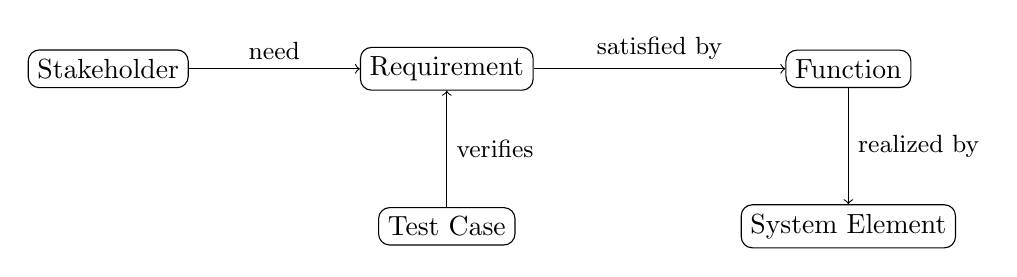
\begin{tikzpicture}[node distance=1.6cm]
\node (stakeholder) [draw, rounded corners] {Stakeholder};
\node (req) [draw, rounded corners, right of=stakeholder, xshift=2.7cm] {Requirement};
\node (func) [draw, rounded corners, right of=req, xshift=3.5cm] {Function};
\node (arch) [draw, rounded corners, below of=func, yshift=-0.4cm] {System Element};
\node (test) [draw, rounded corners, left of=arch, xshift=-3.5cm] {Test Case};
\draw[->] (stakeholder) -- node[above] {\small need} (req);
\draw[->] (req) -- node[above] {\small satisfied by} (func);
\draw[->] (func) -- node[right] {\small realized by} (arch);
\draw[->] (test) -- node[right] {\small verifies} (req);
\end{tikzpicture}


%     \caption{...}
%     \label{fig:kap02-dokumente-modellbeziehungen}
%   \end{figure}
%
% English counterpart of figures/fig_kap02_dokumente_modellbeziehungen.
% =====================================================================

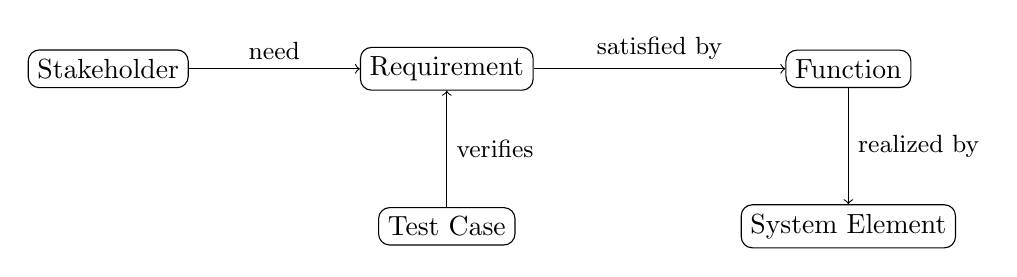
\begin{tikzpicture}[node distance=1.6cm]
\node (stakeholder) [draw, rounded corners] {Stakeholder};
\node (req) [draw, rounded corners, right of=stakeholder, xshift=2.7cm] {Requirement};
\node (func) [draw, rounded corners, right of=req, xshift=3.5cm] {Function};
\node (arch) [draw, rounded corners, below of=func, yshift=-0.4cm] {System Element};
\node (test) [draw, rounded corners, left of=arch, xshift=-3.5cm] {Test Case};
\draw[->] (stakeholder) -- node[above] {\small need} (req);
\draw[->] (req) -- node[above] {\small satisfied by} (func);
\draw[->] (func) -- node[right] {\small realized by} (arch);
\draw[->] (test) -- node[right] {\small verifies} (req);
\end{tikzpicture}

}
  \caption{From document to model relationship: a stakeholder need leads to a requirement, which is satisfied by a function and realized by a system element; a test case verifies the requirement.}
  \label{fig:kap02-dokumente-modellbeziehungen}
\end{figure}

This simple picture already shows the core of MBSE. The point is not to produce many diagrams. The point is to connect system information so that questions become answerable.

\subsection{Traceability}
Traceability lets you follow the links from a requirement to the design and the tests that verify it. You can jump from one piece of information to related ones. From a requirement, you reach functions, components, and tests. From a component, you can see which requirements it satisfies. From a test, you can see which requirement it checks.

For the indoor robot, traceability is especially useful. If the safety requirement is tightened, the team wants to know:

\begin{itemize}
    \item Which functions are affected?
    \item Which sensors and software components are involved?
    \item Which interfaces need to change?
    \item Which tests need to be extended?
    \item What risks arise for cost, schedule, and battery life?
\end{itemize}

Without a model, the team must dig these connections out of documents by hand. With a well-maintained model, at least part of this becomes directly visible.

\section{MBSE in the Robot Project}
For our textbook project, we model the autonomous indoor robot step by step. The model grows together with our understanding. At the start, it does not need to be complete. It should make the most important relationships visible.

\subsection{First Model Structure}
A simple starting structure for the model could look like this:

\begin{itemize}
    \item package \enquote{Stakeholders and Context}
    \item package \enquote{Requirements}
    \item package \enquote{Functions}
    \item package \enquote{System Structure}
    \item package \enquote{Interfaces}
    \item package \enquote{Behavior}
    \item package \enquote{ROS2 Architecture}
    \item package \enquote{Tests and Verification}
\end{itemize}

At this point, a package is just an organizing area. It helps keep the model tidy. Later, we will see how such packages can be set up concretely as SysML v2 files and namespaces.

\subsection{Example Chain: Obstacle Detection}
Consider a typical model chain:

\begin{enumerate}
    \item Stakeholder need: people in the building must not be endangered.
    \item Requirement: the robot must detect obstacles in its path and stop in time.
    \item Function: detect obstacle.
    \item Function: limit movement safely.
    \item System element: lidar sensor.
    \item System element: safety logic.
    \item ROS2 element: topic for sensor data.
    \item ROS2 element: node for obstacle evaluation.
    \item Test case: check stopping behavior for an obstacle at a defined distance.
\end{enumerate}

This chain shows how MBSE bridges from a human need all the way to a technical test. This bridge is exactly what makes MBSE valuable in complex projects. Figure~\ref{fig:kap02-modellkette-traceability} shows this model chain with color coding, from the requirement (blue) through functions and system elements (green) to ROS2 elements (orange) and the test case (gray).

\begin{figure}[H]
  \centering
  \adjustbox{max width=\linewidth,max totalheight=0.6\textheight}{% =====================================================================
% Figure: Model chain: from requirement to test case (obstacle detection)
% Belongs with chapter 2, section "Example Chain: Obstacle Detection"
% (subsection of "MBSE in the Robot Project")
%
% Used in the book, e.g. in chapters_en/02_mbse.tex:
%
%   \begin{figure}[H]
%     \centering
%     % =====================================================================
% Figure: Model chain: from requirement to test case (obstacle detection)
% Belongs with chapter 2, section "Example Chain: Obstacle Detection"
% (subsection of "MBSE in the Robot Project")
%
% Used in the book, e.g. in chapters_en/02_mbse.tex:
%
%   \begin{figure}[H]
%     \centering
%     % =====================================================================
% Figure: Model chain: from requirement to test case (obstacle detection)
% Belongs with chapter 2, section "Example Chain: Obstacle Detection"
% (subsection of "MBSE in the Robot Project")
%
% Used in the book, e.g. in chapters_en/02_mbse.tex:
%
%   \begin{figure}[H]
%     \centering
%     \input{figures_en/fig_kap02_modellkette_traceability}
%     \caption{Color-coded model chain from a stakeholder need, through
%       a requirement, functions, and system elements, to a ROS2 node
%       and a test case.}
%     \label{fig:kap02-modellkette-traceability}
%   \end{figure}
%
% Required packages (already loaded in main_en.tex): tikz
% Required TikZ libraries: positioning, arrows.meta, shadows, calc
% =====================================================================

\input{figures_en/fig_kap02_modellkette_traceability.tikz}

%     \caption{Color-coded model chain from a stakeholder need, through
%       a requirement, functions, and system elements, to a ROS2 node
%       and a test case.}
%     \label{fig:kap02-modellkette-traceability}
%   \end{figure}
%
% Required packages (already loaded in main_en.tex): tikz
% Required TikZ libraries: positioning, arrows.meta, shadows, calc
% =====================================================================

\begin{tikzpicture}[
    every node/.style={font=\small},
    ext/.style={
        rectangle, rounded corners=1.5pt, draw=black!50, thick, dashed,
        minimum width=24mm, minimum height=13mm,
        align=center, fill=white, drop shadow, font=\scriptsize
    },
    req/.style={
        rectangle, rounded corners=1.5pt, draw=black!70, thick,
        minimum width=24mm, minimum height=13mm,
        align=center, fill=blue!12, drop shadow, font=\scriptsize
    },
    part/.style={
        rectangle, rounded corners=1.5pt, draw=green!40!black, thick,
        minimum width=24mm, minimum height=13mm,
        align=center, fill=green!15, drop shadow, font=\scriptsize
    },
    tool/.style={
        rectangle, rounded corners=1.5pt, draw=orange!60!black, thick,
        minimum width=24mm, minimum height=13mm,
        align=center, fill=orange!15, drop shadow, font=\scriptsize
    },
    test/.style={
        rectangle, rounded corners=1.5pt, draw=black!50, thick,
        minimum width=24mm, minimum height=13mm,
        align=center, fill=black!6, drop shadow, font=\scriptsize
    },
    flow/.style={-{Stealth[length=2.2mm]}, thick, black!60}
]

% --- Row 1: stakeholder need to system element lidar sensor ---
\node[ext]  (need) at (1.2,3.5)  {Stakeholder\\Need};
\node[req]  (req)  at (4.0,3.5)  {Requirement};
\node[part] (f1)   at (6.8,3.5)  {Function:\\Detect\\Obstacle};
\node[part] (f2)   at (9.6,3.5)  {Function:\\Limit Movement\\Safely};
\node[part] (lidar)at (12.4,3.5) {System Element:\\Lidar Sensor};

\draw[flow] (need) -- (req);
\draw[flow] (req)  -- (f1);
\draw[flow] (f1)   -- (f2);
\draw[flow] (f2)   -- (lidar);

% --- Row 2: system element safety logic to test case ---
\node[part] (safety) at (12.4,0) {System Element:\\Safety Logic};
\node[tool] (topic)  at (9.6,0)  {ROS2 Topic};
\node[tool] (rosnode)   at (6.8,0)  {ROS2 Node};
\node[test] (tc)     at (4.0,0)  {Test Case};

\draw[flow] (lidar.south)  -- (safety.north);
\draw[flow] (safety) -- (topic);
\draw[flow] (topic)  -- (rosnode);
\draw[flow] (rosnode)   -- (tc);

% --- Legend ---
\node[req, minimum width=6mm, minimum height=4mm, font=\tiny] (leg1) at (1.2,-2.2) {};
\node[right=1mm of leg1, font=\tiny, align=left] (lab1){Requirement};
\node[part, minimum width=6mm, minimum height=4mm, font=\tiny, right=6mm of lab1] (leg2) {};
\node[right=1mm of leg2, font=\tiny, align=left] (lab2){Function / System Element};
\node[tool, minimum width=6mm, minimum height=4mm, font=\tiny, right=6mm of lab2] (leg3) {};
\node[right=1mm of leg3, font=\tiny, align=left] (lab3){ROS2 Element};
\node[test, minimum width=6mm, minimum height=4mm, font=\tiny, right=6mm of lab3] (leg4) {};
\node[right=1mm of leg4, font=\tiny, align=left] (lab4){Test Case};

\end{tikzpicture}


%     \caption{Color-coded model chain from a stakeholder need, through
%       a requirement, functions, and system elements, to a ROS2 node
%       and a test case.}
%     \label{fig:kap02-modellkette-traceability}
%   \end{figure}
%
% Required packages (already loaded in main_en.tex): tikz
% Required TikZ libraries: positioning, arrows.meta, shadows, calc
% =====================================================================

\begin{tikzpicture}[
    every node/.style={font=\small},
    ext/.style={
        rectangle, rounded corners=1.5pt, draw=black!50, thick, dashed,
        minimum width=24mm, minimum height=13mm,
        align=center, fill=white, drop shadow, font=\scriptsize
    },
    req/.style={
        rectangle, rounded corners=1.5pt, draw=black!70, thick,
        minimum width=24mm, minimum height=13mm,
        align=center, fill=blue!12, drop shadow, font=\scriptsize
    },
    part/.style={
        rectangle, rounded corners=1.5pt, draw=green!40!black, thick,
        minimum width=24mm, minimum height=13mm,
        align=center, fill=green!15, drop shadow, font=\scriptsize
    },
    tool/.style={
        rectangle, rounded corners=1.5pt, draw=orange!60!black, thick,
        minimum width=24mm, minimum height=13mm,
        align=center, fill=orange!15, drop shadow, font=\scriptsize
    },
    test/.style={
        rectangle, rounded corners=1.5pt, draw=black!50, thick,
        minimum width=24mm, minimum height=13mm,
        align=center, fill=black!6, drop shadow, font=\scriptsize
    },
    flow/.style={-{Stealth[length=2.2mm]}, thick, black!60}
]

% --- Row 1: stakeholder need to system element lidar sensor ---
\node[ext]  (need) at (1.2,3.5)  {Stakeholder\\Need};
\node[req]  (req)  at (4.0,3.5)  {Requirement};
\node[part] (f1)   at (6.8,3.5)  {Function:\\Detect\\Obstacle};
\node[part] (f2)   at (9.6,3.5)  {Function:\\Limit Movement\\Safely};
\node[part] (lidar)at (12.4,3.5) {System Element:\\Lidar Sensor};

\draw[flow] (need) -- (req);
\draw[flow] (req)  -- (f1);
\draw[flow] (f1)   -- (f2);
\draw[flow] (f2)   -- (lidar);

% --- Row 2: system element safety logic to test case ---
\node[part] (safety) at (12.4,0) {System Element:\\Safety Logic};
\node[tool] (topic)  at (9.6,0)  {ROS2 Topic};
\node[tool] (rosnode)   at (6.8,0)  {ROS2 Node};
\node[test] (tc)     at (4.0,0)  {Test Case};

\draw[flow] (lidar.south)  -- (safety.north);
\draw[flow] (safety) -- (topic);
\draw[flow] (topic)  -- (rosnode);
\draw[flow] (rosnode)   -- (tc);

% --- Legend ---
\node[req, minimum width=6mm, minimum height=4mm, font=\tiny] (leg1) at (1.2,-2.2) {};
\node[right=1mm of leg1, font=\tiny, align=left] (lab1){Requirement};
\node[part, minimum width=6mm, minimum height=4mm, font=\tiny, right=6mm of lab1] (leg2) {};
\node[right=1mm of leg2, font=\tiny, align=left] (lab2){Function / System Element};
\node[tool, minimum width=6mm, minimum height=4mm, font=\tiny, right=6mm of lab2] (leg3) {};
\node[right=1mm of leg3, font=\tiny, align=left] (lab3){ROS2 Element};
\node[test, minimum width=6mm, minimum height=4mm, font=\tiny, right=6mm of lab3] (leg4) {};
\node[right=1mm of leg4, font=\tiny, align=left] (lab4){Test Case};

\end{tikzpicture}

}
  \caption{Color-coded model chain from a stakeholder need, through a requirement, functions, and system elements, to a ROS2 node and a test case.}
  \label{fig:kap02-modellkette-traceability}
\end{figure}

\subsection{Example Chain: Battery Management}
A second chain concerns the battery:

\begin{enumerate}
    \item Stakeholder need: the robot must not stop in the middle of a corridor.
    \item Requirement: the robot must return to the charging station on its own when its battery is low.
    \item Function: monitor battery level.
    \item Function: plan return to charging station.
    \item System element: battery.
    \item System element: battery management.
    \item System element: navigation.
    \item ROS2 element: battery state message.
    \item Test case: check the return to the charging station once a threshold is crossed.
\end{enumerate}

Here, too, you can see that the requirement does not touch just one single component. It connects power supply, software, navigation, charging infrastructure, and testing.

\section{The Benefit of MBSE}
MBSE is not an end in itself. The benefit only appears when the model answers real project questions. The main advantages are traceability, consistency, communication, change analysis, and better preparation for implementation.

\subsection{Traceability}
Traceability means that decisions and connections stay recognizable. If someone asks why the robot has a lidar sensor, the model should not just show \enquote{because we decided so} -- it should show the connection to requirements and functions.

\subsection{Consistency}
A model can help avoid contradictions. If a system element gets renamed, it appears with the same name in every view. If a requirement has no test case, that can be flagged. If a function is not assigned to any component, this becomes an open question.

\subsection{Communication}
Diagrams and structured models help teams talk about the same system. This matters especially in a robot project, because different disciplines are involved. A shared model structure can reduce misunderstandings.

\subsection{Change Analysis}
Changes are normal. MBSE helps you understand the consequences of a change. If the maximum speed increases, that does not just affect the motors. It also affects braking distance, obstacle detection, safety logic, battery life, tests, and possibly approval questions.

\subsection{A Bridge to Implementation}
In this textbook, one point matters especially: the model should later fit the ROS2 architecture. We do not want to model the system and then reinvent everything afterward. We want to understand how requirements, functions, and system elements can map onto nodes, topics, services, parameters, and tests.

\begin{praxisbox}
A SysML function \enquote{detect person} can later map onto a ROS2 node \texttt{object\_detector\_node}. The interface of this function can lead to topics for camera images and detected objects. This creates a traceable connection between the system model and the software structure.
\end{praxisbox}

\section{Limits and Misunderstandings}
MBSE helps manage complexity. But it does not automatically solve every problem. A model can be wrong, outdated, or needlessly complicated. Then it creates more effort than benefit.

\subsection{Misunderstanding 1: MBSE Means Modeling Everything}
A good model does not contain every detail. It contains the details that matter for understanding, decisions, interfaces, risks, and evidence. A model that maps every tiny software parameter can become unmanageable. A model that contains only three pretty pictures is too shallow.

\subsection{Misunderstanding 2: The Model Replaces Communication}
A model supports communication, but it does not replace it. People must still ask questions, make decisions, and clarify assumptions. The model documents and connects the results.

\subsection{Misunderstanding 3: The Tool Does the Engineering}
A SysML v2 tool can check relationships, generate views, and support consistency checks. It does not decide which requirements make sense or which architecture is good. That remains engineering work.

\subsection{Misunderstanding 4: MBSE Is Only for Large Corporations}
MBSE is often associated with large aerospace, automotive, or space projects. The core idea, though, is useful for small projects too. A learning project benefits especially, because it makes relationships visible. You only need to choose the right scope.

\begin{hinweisbox}
For this textbook, the rule is: we model enough to make the connections between SysML v2, MBSE, and ROS2 understandable. We do not model every conceivable detail of the robot.
\end{hinweisbox}

\section{A Pragmatic Start with MBSE}
Beginners should not start MBSE with the goal of building a perfect model right away. A step-by-step start works better.

\subsection{Step 1: Describe Purpose and Context}
First, describe what the system is built for and in which environment it operates. For the robot: indoor spaces, a defined area of a building, people nearby, a charging station, a user interface, and a possible network connection.

\subsection{Step 2: Collect Requirements}
Next, collect the important requirements. They do not need to be perfect at the start. What matters is making them visible, then improving them later. Good requirements are understandable, unambiguous, and testable.

\subsection{Step 3: Derive Functions}
Functions get derived from requirements. If the robot must return to the charging station automatically, it needs functions such as \enquote{monitor battery level,} \enquote{locate charging station,} and \enquote{plan return.}

\subsection{Step 4: Design the Structure}
Next, decide which system elements realize the functions. This is where the first system parts appear (\texttt{part def}, explained in more detail in chapter 3), along with subsystems or components. For the robot, these are, for example, sensors, navigation, power supply, and the user interface.

\subsection{Step 5: Describe Interfaces}
Interfaces should be described early. Who provides which data? Who needs which information? What signals, messages, or energy flows exist?

\subsection{Step 6: Assign Tests}
Tests or other evidence get assigned to the important requirements. This keeps it clear how the team plans to check later whether the system works.

\section{Quality Traits of a Good Model}
An MBSE model is not automatically good just because it is big. Good models share a few practical traits.

\subsection{Clarity}
A new team member should be able to find their way around the model. Names should be self-explanatory. Diagrams should not be overloaded. The structure should be easy to follow.

\subsection{Consistency}
Terms should be used consistently. If a component is called \enquote{Battery Monitor} in one place, \enquote{battery module} in another, and \enquote{Power Node} in a third, misunderstandings follow. For a German textbook, German terms can make sense in the system model, while later ROS2 package names stay technically English.

\subsection{Appropriate Depth}
The model should be neither too coarse nor too detailed. A good question to ask is: \enquote{Does this detail help with a decision, an interface, an implementation, or a check?} If not, it may not belong in a beginner's model.

\subsection{Maintainability}
A model must be maintainable. If every small change requires a lot of manual rework, the model quickly falls out of date. A simple, clear model structure is therefore important.

\subsection{Verifiability}
Important requirements should be connected to evidence. Not every requirement needs a fully worked-out test right away, but it should be clear how its fulfilment will be checked later.

\section{Views and Roles in the Model}
A system model holds a lot of information. Even so, not everyone needs to see all of it all the time. This is why MBSE works with views. A view shows a specific slice of the model for a specific question or role.

This is similar to a map of a building. An architect looks at floor plans, an electrician looks at power lines, the fire department looks at escape routes, and a visitor looks at the site plan. All these views describe the same building, but they show different information.

\subsection{The Project Management View}
Project management cares mainly about progress, risks, open decisions, and the effects of changes. In the MBSE model, this could mean answering questions such as:

\begin{itemize}
    \item Which requirements are still unresolved?
    \item Which requirements have no evidence yet?
    \item Which subsystems are most affected by changes?
    \item Which interfaces are not yet described?
    \item Which risks affect safety, cost, or schedule?
\end{itemize}

For project management, the model is therefore not a technical picture book, but a steering tool. It shows where uncertainty lies.

\subsection{The System Architecture View}
The system architecture view looks at the major building blocks and their relationships. For the robot, this means, for example, the split into sensors, localization, navigation, propulsion, power supply, operation, and safety functions. This view answers questions such as:

\begin{itemize}
    \item Which main systems exist?
    \item Which data and signals flow between them?
    \item Where are the critical interfaces?
    \item Which functions belong to which subsystem?
    \item Which components are responsible for safety-relevant behavior?
\end{itemize}

\subsection{The Software Development View}
Software development cares about data flows, states, sequences, responsibilities, and technical interfaces. In our project, this view becomes especially important later, because we want to connect SysML with ROS2.

A software developer wants to know:

\begin{itemize}
    \item Which ROS2 nodes are needed?
    \item Which topics carry sensor data, status information, or control commands?
    \item Which services or actions fit tasks and navigation?
    \item Which parameters must be configurable?
    \item Which fault states must the software detect?
\end{itemize}

The MBSE model does not yet deliver finished code for this. It does deliver a structured foundation, so the software architecture does not emerge by accident.

\subsection{The Test Team View}
The test team wants to know what must be checked and how tests connect to requirements. One especially important question is whether every central requirement has evidence attached to it.

For the indoor robot, test views could show:

\begin{itemize}
    \item requirements for obstacle detection and matching test scenarios
    \item requirements for battery life and measurement procedures
    \item robot states and tests for state transitions
    \item interfaces between ROS2 nodes and integration tests
    \item fault situations and the expected safe responses
\end{itemize}

This view stops tests from being invented only at the end. Good tests grow alongside the team's understanding of the system.

Figure~\ref{fig:kap02-sichten-auf-modell} summarizes the four views described above once more: all of them access the same model, but look at it from different angles.

\begin{figure}[H]
  \centering
  \adjustbox{max width=\linewidth,max totalheight=0.6\textheight}{% =====================================================================
% Figure: Views onto a shared model
% Belongs with chapter 2, section "Views and Roles in the Model"
%
% Used in the book, e.g. in chapters_en/02_mbse.tex:
%
%   \begin{figure}[H]
%     \centering
%     % =====================================================================
% Figure: Views onto a shared model
% Belongs with chapter 2, section "Views and Roles in the Model"
%
% Used in the book, e.g. in chapters_en/02_mbse.tex:
%
%   \begin{figure}[H]
%     \centering
%     % =====================================================================
% Figure: Views onto a shared model
% Belongs with chapter 2, section "Views and Roles in the Model"
%
% Used in the book, e.g. in chapters_en/02_mbse.tex:
%
%   \begin{figure}[H]
%     \centering
%     \input{figures_en/fig_kap02_sichten_auf_modell}
%     \caption{Four roles look at the same MBSE model of the robot
%       from different angles.}
%     \label{fig:kap02-sichten-auf-modell}
%   \end{figure}
%
% Required packages (already loaded in main_en.tex): tikz
% Required TikZ libraries: positioning, arrows.meta, shadows, calc
% =====================================================================

\input{figures_en/fig_kap02_sichten_auf_modell.tikz}

%     \caption{Four roles look at the same MBSE model of the robot
%       from different angles.}
%     \label{fig:kap02-sichten-auf-modell}
%   \end{figure}
%
% Required packages (already loaded in main_en.tex): tikz
% Required TikZ libraries: positioning, arrows.meta, shadows, calc
% =====================================================================

\begin{tikzpicture}[
    every node/.style={font=\small},
    center/.style={
        rectangle, rounded corners=1.5pt, draw=green!40!black, thick,
        minimum width=34mm, minimum height=14mm,
        align=center, fill=green!15, drop shadow
    },
    role/.style={
        rectangle, rounded corners=1.5pt, draw=black!50, thick, dashed,
        minimum width=32mm, minimum height=13mm,
        align=center, fill=white, drop shadow
    },
    conn/.style={black!45, dashed, thick}
]

% --- Center ---
\node[center] (modell) at (6,3) {MBSE Model\\of the Robot};

% --- Four views/roles ---
\node[role] (pl)  at (6,5.65)  {Project Management\\(progress, risks)};
\node[role] (arch) at (11,3) {System Architecture\\(building blocks, interfaces)};
\node[role] (sw)  at (5.99,0.35)  {Software Development\\(nodes, topics)};
\node[role] (test) at (1,3)  {Test Team\\(requirements $\leftrightarrow$ tests)};

\draw[conn] (modell) -- (pl);
\draw[conn] (modell) -- (arch);
\draw[conn] (modell) -- (sw);
\draw[conn] (modell) -- (test);

% --- Legend ---
\node[center, minimum width=6mm, minimum height=4mm, font=\tiny] (leg1) at (2.74,-1.34) {};
\node[right=1mm of leg1, font=\tiny, align=left] (lab1){shared model};
\node[role, minimum width=6mm, minimum height=4mm, font=\tiny, right=6mm of lab1] (leg2) {};
\node[right=1mm of leg2, font=\tiny, align=left] (lab2){view/role on the model};

\end{tikzpicture}


%     \caption{Four roles look at the same MBSE model of the robot
%       from different angles.}
%     \label{fig:kap02-sichten-auf-modell}
%   \end{figure}
%
% Required packages (already loaded in main_en.tex): tikz
% Required TikZ libraries: positioning, arrows.meta, shadows, calc
% =====================================================================

\begin{tikzpicture}[
    every node/.style={font=\small},
    center/.style={
        rectangle, rounded corners=1.5pt, draw=green!40!black, thick,
        minimum width=34mm, minimum height=14mm,
        align=center, fill=green!15, drop shadow
    },
    role/.style={
        rectangle, rounded corners=1.5pt, draw=black!50, thick, dashed,
        minimum width=32mm, minimum height=13mm,
        align=center, fill=white, drop shadow
    },
    conn/.style={black!45, dashed, thick}
]

% --- Center ---
\node[center] (modell) at (6,3) {MBSE Model\\of the Robot};

% --- Four views/roles ---
\node[role] (pl)  at (6,5.65)  {Project Management\\(progress, risks)};
\node[role] (arch) at (11,3) {System Architecture\\(building blocks, interfaces)};
\node[role] (sw)  at (5.99,0.35)  {Software Development\\(nodes, topics)};
\node[role] (test) at (1,3)  {Test Team\\(requirements $\leftrightarrow$ tests)};

\draw[conn] (modell) -- (pl);
\draw[conn] (modell) -- (arch);
\draw[conn] (modell) -- (sw);
\draw[conn] (modell) -- (test);

% --- Legend ---
\node[center, minimum width=6mm, minimum height=4mm, font=\tiny] (leg1) at (2.74,-1.34) {};
\node[right=1mm of leg1, font=\tiny, align=left] (lab1){shared model};
\node[role, minimum width=6mm, minimum height=4mm, font=\tiny, right=6mm of lab1] (leg2) {};
\node[right=1mm of leg2, font=\tiny, align=left] (lab2){view/role on the model};

\end{tikzpicture}

}
  \caption{Four roles look at the same MBSE model of the robot from different angles.}
  \label{fig:kap02-sichten-auf-modell}
\end{figure}

\section{From the MBSE Model to the ROS2 Architecture}
One central goal of this textbook is to connect SysML v2, MBSE, and ROS2. It is therefore important to understand early on how a system model can lead to a later software structure.

This transition does not happen automatically. A SysML system element does not turn into a ROS2 node by magic. But the model can systematically prepare which software units make sense and how they communicate with each other.

\subsection{Functions as a Starting Point}
Functions come first. Functions describe what the system must do. For the robot, these are, for example, \enquote{sense the environment,} \enquote{determine position,} \enquote{plan a route,} \enquote{avoid obstacles,} \enquote{detect people,} and \enquote{monitor battery level.}

These functions can later map onto software building blocks. Not every function automatically becomes its own node. Sometimes several functions get grouped into one node. Sometimes one function gets split across several nodes. Modeling helps the team make this decision deliberately.

\subsection{Data Flows as Preparation for Topics}
ROS2 systems often communicate over topics. A topic carries messages from one sender to one or more receivers. In the MBSE model, data flows can be prepared before concrete topic names get decided.

Examples:

\begin{itemize}
    \item The camera sends image data to people detection.
    \item The lidar sends distance data to obstacle evaluation.
    \item Localization sends the current pose to navigation.
    \item Navigation sends speed targets to drive control.
    \item Battery management sends charge level to mission planning.
\end{itemize}

Later, these can become ROS2 topics such as \texttt{/camera/image}, \texttt{/scan}, \texttt{/robot\_pose}, \texttt{/cmd\_vel}, or \texttt{/battery\_state}. The exact names are technical decisions. But the underlying communication structure can already become visible in the model.

\subsection{States as a Basis for Control Logic}
An autonomous robot has operating states. Examples are \enquote{ready,} \enquote{task active,} \enquote{navigating,} \enquote{obstacle detected,} \enquote{returning,} \enquote{charging,} and \enquote{fault.} These states can be modeled in SysML and help later during software development.

Without a state model, control logic often ends up scattered through the code. After a while, no one knows exactly when the robot may drive, when it must stop, or how it recovers from a fault state. A state model creates a shared foundation.

\subsection{Tests as the Link Between Model and Code}
Tests form an important bridge between the model and the implementation. If a requirement in the model is linked to a test case, the later code can be checked specifically against this expectation.

Example:

\begin{enumerate}
    \item Requirement: the robot must return to the charging station when its battery is low.
    \item Model function: trigger return to the charging station.
    \item ROS2 node: \texttt{battery\_monitor\_node} reports a low charge level.
    \item ROS2 node: \texttt{navigation\_node} receives the \enquote{charging station} target.
    \item Test: simulated battery level drops below the threshold, and a return target is then set.
\end{enumerate}

In this way, a functional expectation becomes a testable technical implementation.

\section{Typical Mistakes When Starting with MBSE}
MBSE, too, can be applied the wrong way. Especially at the start, a few warning signs help.

\subsection{Mistake 1: Diagrams Without Model Content}
The team draws nice diagrams, but the elements are not named cleanly, not reused, and not linked. This produces only a prettier form of document-centric development.

\subsection{Mistake 2: Too Many Details Too Early}
Beginners sometimes try to model every cable, every software class, and every parameter right away. This makes the model large before the basic structure is understood. It works better to start with requirements, main functions, main systems, and critical interfaces.

\subsection{Mistake 3: No Model Maintenance}
A model is only useful if it is maintained. If architecture decisions change in the code but never flow back into the model, the model loses its value. The project must therefore make clear which parts of the model are maintained as a binding source of truth.

\subsection{Mistake 4: Unclear Modeling Rules}
If every team member models differently, disorder follows. Even simple rules help: consistent names, a clear package structure, defined relationship types, and limited diagram sizes.

\subsection{Mistake 5: Model and Implementation Become Separate Worlds}
The model must not run alongside development like a box-ticking exercise. It must answer questions that really come up in the project. In this textbook, the connection to the ROS2 architecture therefore matters: the model should not just explain, it should prepare the implementation.

\section{Summary}
\gls{mbse} carries the ideas of systems engineering into a model-based way of working. Instead of spreading project knowledge across many loose documents, key information gets structured and linked within a system model. The model holds requirements, functions, structure, interfaces, behavior, tests, assumptions, and decisions.

The most important point is not drawing diagrams, but building relationships. A requirement does not stand alone. It connects to stakeholders, functions, system elements, interfaces, and tests. This traceability is exactly what makes MBSE valuable.

For the autonomous indoor robot, this means: we can think from a user's need, through requirements and functions, all the way to the later ROS2 architecture. The model becomes a bridge between understanding the problem, SysML v2 modeling in the Syside Editor, and technical implementation.

\section{Review Questions}
\begin{enumerate}
    \item What does Model-Based Systems Engineering mean?
    \item How does a model differ from a simple diagram image?
    \item Why does document-centric development become problematic in more complex projects?
    \item What kinds of information can an MBSE model contain?
    \item What is traceability?
    \item Why does traceability matter for requirements and tests?
    \item Name three typical model relationships in the robot project.
    \item Why doesn't MBSE replace the source code?
    \item Why doesn't MBSE replace communication within the team?
    \item What advantages does MBSE offer when things change?
    \item What would be an example of modeling that is too detailed?
    \item Which packages would you create for a first model of the indoor robot?
\end{enumerate}

\section{Exercises}
\begin{uebungbox}
\textbf{Exercise 1: Spot Document Chaos}\\
Make a list of five documents or information sources that could arise in a typical robot project. For each source, describe the risk that appears if it is not kept up to date.
\end{uebungbox}

\begin{uebungbox}
\textbf{Exercise 2: Build a Model Chain}\\
Build a simple chain from stakeholder need, requirement, function, system element, and test case for the automatic return to the charging station.
\end{uebungbox}

\begin{uebungbox}
\textbf{Exercise 3: Link Requirements}\\
Choose three requirements for the indoor robot. For each requirement, assign at least one function, one possible system element, and one test case.
\end{uebungbox}

\begin{uebungbox}
\textbf{Exercise 4: Limit Model Scope}\\
Note down ten possible pieces of information about the robot. For each one, decide whether it belongs in a beginner's MBSE model or can stay outside it for now. Give a short reason for each decision.
\end{uebungbox}

\begin{uebungbox}
\textbf{Exercise 5: Change Analysis}\\
Suppose the robot's maximum speed increases from 0.8 m/s to 1.2 m/s. Describe which requirements, functions, components, interfaces, and tests this could affect.
\end{uebungbox}

\section{Further Reading}
For getting started with MBSE, practice-oriented introductions to SysML are especially helpful, because they treat modeling not abstractly but through requirements, architecture, and behavior. Particularly recommended are the works on SysML already cited in this project, for example Delligatti \cite{delligatti2014} and Friedenthal, Moore, and Steiner \cite{friedenthal2014}.

Beyond that, further reading on systems engineering, requirements management, verification and validation, and model-based development of cyber-physical systems pays off. For later technical implementation, the ROS2 documentation \cite{ros2docs} is also important, because it shows how software architectures with nodes, topics, services, actions, and parameters are built in practice.
